\chapter{تثبيت الـ\textenglish{SDL}}

ابتداءً من الآن، إنتهت الدروس النظرية ! لأننا سنمرّ إلى مرحلة مهمّة، و سنستمتع بالتطبيق بالاستعانة بمكتبة نسميها
\underline{\textenglish{SDL}}.

في الفصول السابقة كنا قد تطرّقنا تقريباً لكلّ أساسيات اللغة
\textenglish{C}،
لكن تبقى هناك دائماً بعض التفاصيل الصعبة نوعاً ما لنكتشفها. سأقول لك بأنه يُمكن لهذا الكتاب أن يتوقّف هنا مخبرا إيّاك : "نعم لقد تعلّمت البرمجة بلغة 
\textenglish{C}"،
لكني متأكّد بأن الجميع سيشاركني الرأي لو قلت بأن المُبرمج سيحسّ نفسه دائماً مبتدئاً مادام لم "يخرج" من الكونسول !

الـ\textenglish{SDL}
هي مكتبة تُستخدم خاصّة لإنشاء ألعاب ثنائية الأبعاد. سنتعرّف في هذا الفصل على هذه المكتبة و نتعلّم كيف نقوم بتثبيتها.

نسمي هذا النوع من المكتبات بمكتبات الطرف الثالث 
(\textenglish{Third party libraries}).
يجب أن تعرف أنه يوجد نوعان من المكتبات :

\begin{itemize}
	\item \textbf{المكتبة القياسية}
	(\textenglish{Standard library}) :
	و هي المكتبة القاعدية التي تعمل على كلّ أنظمة التشغيل (من هنا تم استنباط الكلمة 
	\textenglish{standard})
	و هي تسمح بالقيام بأمور بسيطة كـ\InlineCode{printf}.
	هذه المكتبات يتمّ تسطيبها تلقائيّا عند تثبيتك للبيئة التطويرية و المترجم.
	
	خلال الجزئين الأوّلين من هذا الكتاب، كناّ قد استعملنا المكتبة القياسيّة فقط
(\InlineCode{stdlib.h}، \InlineCode{stdio.h}، \InlineCode{string.h}، \InlineCode{time.h} \dots).
	لم نقم بدراستها بالتفصيل لكنّا جرّبنا منها جزءً كبيراً. إن كنت تريد معرفة المزيد عن هذا النوع من المكتبات أجْرِ بحثاً في 
	\textenglish{Google}،
	مثلاً بكتابة
	"\textenglish{C standard library}"،
	و ستجد نماذج الدوال في هذه المكتبة، بالإضافة إلى شرح قصير حول دور كلّ دالة.
	\item \textbf{مكتبات الطرف الثالث}
	(\textenglish{Third party libraries}):
	هي مكتبات لا يتم تثبيتها تلقائيا. و إنّما يجب عليك تنزيلها من الأنترنت و تثبيتها بنفسك على حاسوبك.

	على عكس المكتبات القياسية، التي تكون بسيطة نسبيّا و تحتوي على عدد قليل من الدوال، فإنه توجد الآلاف من مكتبات الطرف الثالث، و التي تمت كتابتها من طرف مبرمجين آخرين. بعضها جيّدة، و أخرى أقل، بعضها مدفوع، و بعضها الآخر مجاني، إلخ. الأمر المثالي هو إيجاد مكتبة جيّدة و مجانية في نفس الوقت !
\end{itemize}

إنه لمن المستحيل أن أضع لك درساً يشرح كل المكتبات الموجودة. حتّى لو أمضيت حياتي كلّها 24 ساعة / 24، لن أستطيع !\\
لذا سأقدّم لك مكتبة واحدة فقط مكتوبة بالـ\textenglish{C} و مُستعملة من طرف مبرمجين مثلك. 

هذه المكتبة تدعى 
\textit{\textenglish{SDL}}.
السؤال المطروح هو لماذا اخترت هذه المكتبة بالضبط ؟ ما الذي يميّزها عن باقي المكتبات ؟\\
هذه أسئلة سأبدأ في الإجابة عليها إنطلاقاً من الآن.

\section{لماذا نختار الـ\textenglish{SDL} ؟}

\subsection{اختيار مكتبة ليس بالأمر السهل !}

كما قلت لك الآن، توجد الآلاف من المكتبات للتنزيل.\\
بعضها بسيط، و بعضها كبير جداً لدرجة أن درساً كهذا لا يكفي أن يشرحها كلّها !

الاختيار صعب. لكنّي اخترت هذه المكتبة، التي هي نوعاً ما سهلة الاستعمال، كبداية. ستكون هذه إذا أوّل مكتبة تقوم باستعمالها (إذا لم نحسب المكتبة القياسية).

إنه من الواضح أن أغلب القرّاء يريدون معرفة كيفية فتح نوافذ، إنشاء لعبة، إلخ. و لكن إن كنت تحب الكونسول فيمكننا الاستمرار فيها لوقت أطول، إذا أردت، لا ؟ إذا لدينا هنا بعض الفضول ! \\
أودّ كثيراً أن أريك كيف تعمل كلّ هذه الأمور، لكننا سنحاول أن نتطرّق إليها خطوة بخطوة، و بالنسبة للأعمال التطبيقية، فلدينا عملان تطبيقيان لهذا الجزء من الكتاب !

لقد اخترت لك مكتبة سهلة و قوية، ستكون كبداية لك في تحقيق (تقريبا) أحلامك المتعلّقة بالواجهة الرسومية، و من دون تعب (حسناً، كلّ شيء نسبيّ بالطبع !).
\subsection{الـ\textenglish{SDL}، اختيار جيّد !}

سنقوم الآن بدراسة هذه المكتبة. لماذا اخترتها هي و ليس أخرى ؟

\begin{figure}[H]
	\centering
	
\includegraphics[width=0.4\textwidth]{Chapter_III-1_SDL}
\end{figure}

\begin{itemize}
	\item \textbf{هي مكتبة مكتوبة بلغة
	\textenglish{C}} :
	 أي أنه بإمكان المبرمجين أن يستعملوها في برامجهم المكتوبة بالـ\textenglish{C}.
	 و كما هو الحال بالنسبة لأغلب المكتبات المكتوبة بالـ\textenglish{C}،
	 يمكن استعمالها في لغة الـ\textenglish{C++}
	 بالإضافة إلى لغات برمجية أخرى.
	 \item \textbf{هي مكتبة حُرّة و مجانية} :
و هذا كي لا تضطرّ لدفع أي ثمن مقابل استعمالك ما سأقدّمه لك في بقيّة الكتاب. على عكس ما قد نعتقد، إيجاد مكتبة جيدة و مجانية ليس أمراً صعباً كثيراً، فقد انتشرت كثيراً في أيامنا هذه. المكتبة الحرة هي ببساطة مكتبة يمكنك الحصول على الشفرة المصدرية الخاصة بها. في حالتنا هذه، رؤية الشفرة ليس مُهمّا بالنسبة لنا. لكن كونها حرة يفتح لنا الباب من أجل ميزات أخرى أهمّها المداومة (أي أنه إن توقف صاحب المكتبة عن تطويرها، يُمكن لمبرمجين آخرين أن يكملوا عمله)، بالإضافة إلى مجّانيّتها غالبا. هذا يعني عدم إمكانيّة اختفاء المكتبة في يوم من الأيام.
	 \item \textbf{يُمكنك إنشاء برامج تجارية ذات ملكية خاصة بفضل هذه المكتبة}.
	 قد أكون قد تسرّعت بهذا الكلام، لكنّه يجب اختيار مكتبة حرّة تمنحك الحريّة الأقصى. الحقيقة أنه يوجد نوعان من المكتبات الحُرة :
	 
	 \begin{itemize}
	 	\item المكتبات تحت 
	 	\textbf{رخصة \textenglish{GPL}} :
	 	 مكتبات مجانية، و يمكنك رؤية الشفرة المصدرية الخاصة بها، لكن بشرط أن تقوم أنت كذلك بنشر الشفرة المصدرية الخاصة بالبرنامج الذي أنشأته باستخدامها.
	 	\item المكتبات تحت 
	 	\textbf{رخصة \textenglish{LGPL}} :
	 	مثل سابقتها، لكن ليس عليك أن تنشر الشفرة المصدرية الخاصة بالبرنامج. أي أنه يمكنك بها إنشاء برامج مملوكة.
	 \end{itemize}
 	
 	\begin{information}
بالرغم من أنه يمكنك قانونيّا عدم نشر الشفرة المصدرية الخاصة بالبرنامج، إلا أنني أنصحك بذلك. فبهذا يمكنك أن تأخذ رأي المبرمجين الأكثر تمرّساً منك. و هذا يسمح لك بالتحسّن. بعد هذا، فإن إنشاء برنامج حُر أو ذو ملكية خاصة، يرجع لطبيعة تفكير كل شخص. لن أدخل في نقاش بخصوص هذا الموضوع، لكن فلتعلم أن كلّ النوعين له مميزاته و مساوءه.
 	\end{information}

 	\item هي مكتبة
 	\textbf{متعددة المنصّات} 
 	(\textenglish{Multi-platform}) :
 	سواء كنت على
 	\textenglish{Windows}،
 	\textenglish{\mbox{Mac OS X}}
 	أو
 	\textenglish{\mbox{GNU/Linux}}،
 	ستعمل لديك هذه المكتبة. و الحقيقة أن هذه نقطة قوّة يراها المبرمجون بالمكتبة : يمكنها أن تعمل على عدد كبير جداً من أنظمة التشغيل، فعلى غرار 
 	 	\textenglish{Windows}،
 	\textenglish{\mbox{Mac OS X}}
 	و
 	\textenglish{\mbox{GNU/Linux}}،
 	فهي تشتغل أيضاً على 
 	\textenglish{Atari}، \textenglish{Amiga}، \textenglish{Symbian}، \textenglish{Dreamcast} \dots
 	إلخ. أي أنه بالإمكان لبرامجك أن تعمل حتى على أجهزة 
 	\textenglish{Atari}
 	القديمة ! مع ذلك يجب القيام ببعض التعديلات و ربّما استخدام مترجم خاص. لن أدخل في التفاصيل هنا.
 	\item أخيرا، فإن هذه المكتبة تسمح لك بالقيام بالكثير من 
 	\textbf{الأمور الممتعة}
 	التي سنتعرّف إليها من خلال الفصول القادمة. لا أقول أنّ مكتبة رياضيّاتيّة قادرة على حلّ معادلات من الدرجة الرابعة ليست ممتعة، لكنّي سأركّز على أن يكون هذا الدرس سهلا قدر الإمكان لكيّ يحثّك على البرمجة.
\end{itemize}

هذه المكتبة ليست مخصصة فقط لإنشاء ألعاب الفيديو. سأعترف بأن معظم البرامج التي تمت كتابتها بهذه المكتبة، هي عبارة عن ألعاب، لكن هذا لا يعني أنك مجبر لاستعمالها من أجل ذلك. كما نعلم، كلّ شيء ممكن بالعمل و الاجتهاد. كنت قد رأيت من قبل محرر نصوص تمت برمجته بالـ\textenglish{SDL}،
على الرغم من أنّه هناك مكتبات أخرى أحسن لهذا الغرض. إن كنت تريد برمجة واجهة رسومية تقليديّة تسمح بإظهار نافذة، زر، قائمة، إلخ. فأنا أنصحك إذا بالتوجّه إلى المكتبة 
\textenglish{GTK+}.

\subsection{الإمكانيات المتاحة بالـ\textenglish{SDL}}

المكتبة
\textenglish{SDL}
هي مكتبة منخفضة المستوى. هل تتذكر أول الكتاب حينما حدّثتك عن لغات البرمجة عالية المستوى و لغات البرمجة منخفضة المستوى ؟ هذا ينطبق على المكتبات أيضاً.

\begin{itemize}
	\item \textbf{المكتبات منخفضة المستوى} : 
	تحتوي على دوال قاعدية جدّا. يوجد عدد قليل من هذه الدوال لأنّه يمكننا القيام بكلّ شيء بها. و هذه الدوال لبساطتها تكون سريعة جدّا. لهذا فالبرامج المنشأة بهذا النوع من المكتبات تكون عادة الأسرع.
	\item \textbf{المكتبات عالية المستوى} : 
	تحتوي على الكثير من الدوال التي تسمح بالقيام بالكثير من المهام. هذا يجعلها أبسط من ناحية الاستخدام.
	
	لكن هذا النوع من المكتبات يكون عادة "كبيرا"، و ليس من السهل دراستها و معرفتها بأكملها. كما أنها قد تكون أثقل من المكتبات منخفضة المستوى (لكنّ هذا قد لا يكون واضحا).
\end{itemize}

على العموم، لا يمكننا القول بأن "مكتبة منخفضة المستوى هي أحسن من مكتبة عالية المستوى" أو العكس. فكلّ منهما لها مميزات و مساوئ. الـ\textenglish{SDL}
التي سنقوم بدراستها، تنتمي إلى المكتبات منخفضة المستوى.

يجب إذا أن تتذكر بأن الـ\textenglish{SDL}
تقدّم دوالا قاعدية. يمكنك إذا الرسم بيكسلا ببيكسل، رسم مستطيل أو إظهار صور. هذا كلّ شيء، و صدّقني أنّ هذا كافٍ.

\begin{itemize}
	\item بتحريك صورة، يمكنك أن تقوم بتحريك شخصيّة.
	\item بإظهار العديد من الصور الواحدة تلو الأخرى بسرعة، يمكنك إنشاء تحريك
	(\textenglish{Animation}).
	\item بوضع العديد من الصور، الواحدة بجنب الأخرى، يكون باستطاعتك إنشاء لعبة حقيقيّة.
\end{itemize}

كمثال عن لعبة تم صنعها بالـ\textenglish{SDL}،
اعلم أنّ اللعبة الشهيرة
"\textenglish{Civilisation : Call to power}"،
تم دعمها في نظام اللينكس لاحقاً باستخدام الـ\textenglish{SDL}.

\begin{figure}[H]
	\centering
	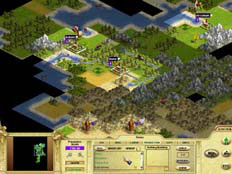
\includegraphics[width=0.5\textwidth]{Chapter_III-1_Game}
\end{figure}

يجب أن تعلم أنّ جودة اللعبة تعود إليك و إلى الفريق الذي تعمل معه. إن كان لديك مصمم موهوب، فيمكنك صنع لعبة أجمل.

الشيء الوحيد الذي يحدّ الـ\textenglish{SDL}
هو أنها تقتصر على الألعاب ثنائية الأبعاد، و لم تُنشأ من أجل الألعاب ثلاثية الأبعاد. هذه أمثلة على ألعاب يمكن تحقيقها بالـ\textenglish{SDL}
(ليست سوى قائمة صغيرة، كلّ شيء ممكن مادام ثنائيّ الأبعاد) :

\begin{itemize}
	\item \textenglish{Breakout}
	\item \textenglish{Bomberman}
	\item \textenglish{Tetris}
	\item ألعاب المنصّات :
	\textenglish{Super Mario Bros}، \textenglish{Sonic}، \textenglish{Rayman}، \dots
	\item \textenglish{RPG} ثنائية الأبعاد :
	\textenglish{Zelda}،
	الأجزاء الأولى للعبة
	\textenglish{Final Fantasy}،
	إلخ.
\end{itemize}
لا يمكن وضع لائحة كاملة، الأمر يعود فقط للقدرة على التخيّل. و صدّقني بأنك قادر على برمجة ألعاب فائقة الروعة. فلقد رأيت أحد القرّاء ينشئ تهجينا بين
\textenglish{Breakout}
و
\textenglish{Tetris}.

فلنعد إلى الأرض و لنمسك خيط هذا الفصل. سنقوم الآن بتسطيب المكتبة، لنتمكّن من التقدّم في العمل.

\section{تنزيل الـ\textenglish{SDL}}

الموقع الرسمي للمكتبة 
\textenglish{SDL}
سيصبح قريبا الوجهة الّتي نقصدها كثيرا. هناك، يوجد كلّ ما تحتاجه، بدءً من المكتبة نفسها و مرورا إلى التوثيق 
(\textenglish{Documentation})
الخاص بها.

\url{http://www.libsdl.org/}

إذهب إلى اللائحة
\textenglish{Download}
المتواجدة على يسار الصفحة الرئيسية للموقع.\\
اختر النسخة الأحدث الّتي تجدها
(\textenglish{SDL 1.2}
عندما كتبت هذه السطور).

صفحة التنزيل مجزّأة إلى عدة أجزاء. 

\begin{itemize}
	\item \textbf{الشفرة المصدرية}
	(\textenglish{Source code}) :
هنا يمكنك تحميل الشفرة المصدرية الخاصة بالمكتبة. أدري أن القراء فضوليون ليعرفوا كيف تعمل المكتبة من الداخل، لكنّ هذا لن يفيدنا. الأسوأ هو أنّه سيقوم بإلهائك عن هدفنا الرئيسي.
	\item \textbf{مكتبات وقت التشغيل}
	(\textenglish{Runtime libraries}) :
	هي الملفات التي تحتاج إلى تقديمها مع الملف التنفيذي حين تريد أن تعطي برنامجك لشخص آخر. بالنسبة للويندوز، أنا أتكلم عن الملف 
	\InlineCode{SDL.dll}.
	هذا الأخير يجدر به أن يتواجد إما :
	
	\begin{itemize}
		\item بنفس المجلّد الذي يحتوي الملف التنفيذي
		(أنا أنصحك بهذا). الأحسن دائما هو أن تعطي الـ\textenglish{DLL}
		مع الملف التنفيذي و تبقيهم في نفس المجلد. إذا وضعت الـ\textenglish{DLL}
		في المجلّد الخاص بالويندوز، لن يكون عليك إلحاق الـ\textenglish{DLL}
		مع كلّ مجلّد يحتوي البرنامج
		\textenglish{SDL}.
		و مع ذلك قد تحدث بعض المشاكل في حال ما قمت بمسح نسخة أحدث من الـ\textenglish{DLL}.
		\item في المجلّد
		\InlineCode{C:\textbackslash Windows}.
	\end{itemize}
	
	\item \textbf{مكتبات التطوير}
	(\textenglish{Development libraries}) :
	هي الملفات
	\InlineCode{.a}
	(أو
	\InlineCode{.lib}
	بالنسبة للـ\textenglish{Visual})
	و الملفات 
	\InlineCode{.h}
	التي تسمح بإنشاء برامجك
	\textenglish{SDL}.
	هذه الملفات ليست مفيدة إلا بالنسبة إليك أنت فقط المبرمج. أي أنه ليس عليك تقديمها مع ملفات البرنامج حين تنتهي من هذا الأخير.
\end{itemize}

إذا كنت تعمل في الويندوز، فسأعطيك ثلاثة نسخ، و ذلك حسب المترجم الخاص بك :

\begin{itemize}
	\item \textenglish{VC6} :
	بالنسبة للذين يستخدمون النسخ القديمة غير المجانية من
	\textenglish{Visual studio}
	(لا أعتقد أن هناك من القرّاء من لازال يستعمل هذه النسخ). ستجد فيها على أي حال الملفات
	\InlineCode{.lib}.
	\item \textenglish{VC8} :
	 بالنسبة للذين يستعملون 
	\textenglish{Visual Studio 2005 Express}
	أو نسخة أحدث، ستجد فيها الملفات
	\InlineCode{.lib}.
	\item \textenglish{mingw32} :
	بالنسبة للذين يستعملون 
	\textenglish{Code::Blocks}
	(ستجدون فيها إذا الملفات
	\InlineCode{.a}).
\end{itemize}

الشيء الخاص هنا، هو أن "مكتبات التطوير" تحتوي كل الملفات
\InlineCode{.h}
و الملفات
\InlineCode{.a}
(أو
\InlineCode{.lib})
بالطبع، لكنها تحتوي أيضاً الملف 
\InlineCode{SDL.dll}
و ملفات التوثيق الخاصة بالـ\textenglish{SDL} !\\
باختصار، كلّ ما عليك تنزيله هو "مكتبات التطوير"، فكلّ ما تحتاجه يتواجد بداخلها.

\begin{critical}
لا تخطئ في الرابط ! قم باختيار الـ\textenglish{SDL}
في قسم
"\textenglish{Development libraries}"
و ليس من قسم
"\textenglish{Source code}" !
\end{critical}

\begin{question}
ما هو التوثيق 
(\textenglish{Documentation}) ؟
\end{question}

التوثيق هو قائمة تحوي اللائحة الكاملة للدوال الخاصة بمكتبة معيّنة. و كل هذه الملفات تكون مكتوبة بالانجليزية (حتى لو كان كاتبوها مبرمجين فرنسيين). هذا سبب آخر يدفعك للتقدّم في لغة
\textenglish{Shakespeare} !

محتوى ملفات التوثيق  ليس عبارة عن درس، بل هي عادة موجزة. الشيء الإيجابي بالنسبة لدرس، هي أنّها تحتوي قائمة لكل الدوال الموجودة،  فهي إذا المرجع للمبرمج.\\
في كثير من الأحيان ستجد مكتبات بدون دروس تشرح كيفية عملها. و هنا لا يبقى لك سوى التوثيق الّذي نسميه عادة
"\textenglish{doc}"،
و يجب عليك تدبّر أمرك بهذا فقط (حتّى لو كان هذا صعبا أحيانا عندما تبدأ من دون أيّة مساعدة). المبرمج الحقيقيّ هو من يتمكّن من إيجاد ضالّته في الـ"\textenglish{doc}".

لحدّ الآن، أنت لست بحاجة إلى التوثيق الخاص بالـ\textenglish{SDL}
لأنني أنا من سيشرح لك كيفية عملها. لكن بما أنني غير قادر على أن أشرح لك كل الدوال التي بها، ستحتاج إلى قراءة التوثيق لاحقا. 

ملفّات التوثيق توجد أصلاً في الحزمة
"\textenglish{Development libraries}"
كما سبق و ذكرت، لكن بإمكانك تنزيلها وحدها من القائمة
\InlineCode{Documentation} / \InlineCode{Downloadable}.\\
أنصحك أن تجمع ملفات
\textenglish{HTML}
الخاصة بالتوثيق في مجلّد خاصّ (اسمه مثلاً
\InlineCode{Doc SDL})
ثم إنشاء اختصار إلى الفهرس
\InlineCode{index.html}.
و الهدف من هذا هو الوصول إلى هذه الملفات بشكل أسرع حينما تحتاج إليها.

\section{إنشاء مشروع \textenglish{SDL} : \textenglish{Windows}}

تثبيت مكتبة قد يكون أكثر صعوبة قليلاً مما تعوّد عليه الجميع. هنا لا يوجد تثبيت تلقائيّ يطلب منك أن تنقر "التالي"، "التالي"، "التالي"، "إنتهى".

الحقيقة أن تثبيت مكتبة أمر صعب على المبتدئين. لكن لأقوم برفع المعنويات فإن تسطيب مكتبة 
\textenglish{SDL}
أمر سهل جداً مقارنة بتسطيب مكتبات أخرى أتيحت ليّ فرصة استخدامها من قبل (هناك من يتم إعطاؤك منها الشفرة المصدرية فقط، بينما أنت تتولى أمر الترجمة !).

و الحقيقة أن كلمة "تثبيت" ليست الملائمة هنا. لن نقوم بتثبيت أي شيء، فقط نريد أن نصل إلى الكيفية التي ننشئ فيها مشروع 
\textenglish{SDL}
في البيئة التطويرية الخاصة بنا.\\
ستختلف كيفية التعامل حسب البيئة التطويرية التي تستعملها. سأقوم بتقديم الطريقة الخاصة بكلّ بيئة من بيئات التطوير التي قدّتمها في بداية الكتاب، و هكذا كي يستطيع الجميع المتابعة.

سأعرض الآن كيف ننشئ مشروع
\textenglish{SDL}
في كلّ واحد من البيئات الثلاث السابقة.

\subsection{تسطيب الـ\textenglish{SDL} في \textenglish{Code::Blocks}}

\subsubsection{استخراج ملفات الـ\textenglish{SDL}}

افتح الملف المضغوط
"\textenglish{Development Libraries}"
الذي قمت بتنزيله.\\
هذا الملف هو بامتداد
\InlineCode{.zip}
بالنسبة للـ\textenglish{Visual}
و 
\InlineCode{.tar.gz}
بالنسبة للـ\textenglish{mingw32}
(يلزمك برنامج مثل 
\textenglish{Winrar}
أو
\textenglish{7-Zip}
لكي تقوم بفك الضغط عن الملفات ذات الصيغة 
\InlineCode{.tar.gz}).

الملف المضغوط يحتوي العديد من المجلّدات الداخلية، و هذه هي الملفات التي تهمّنا :

\begin{itemize}
	\item \InlineCode{bin} :
	يحتوي الملف 
	\InlineCode{.dll}
	الخاص بالـ\textenglish{SDL}.
	\item \InlineCode{docs} :
	يحتوي الملفات التوثيقيّة الخاصة بالـ\textenglish{SDL}.
	\item \InlineCode{include} :
	يحتوي الملفات الرأسية
	\InlineCode{.h}.
	\item \InlineCode{lib} :
	يحتوي الملفات 
	\InlineCode{.lib}
	(أو
	\InlineCode{.a}
	بالنسبة لـ\textenglish{Code::Blocks})
\end{itemize}

يجب عليك استخراج كل الملفات و المجلّدات الداخلية ووضعها في مكان ما بالقرص الصلب لحاسوبك، يمكنك مثلا وضعها في مجلد خاص بـ\textenglish{SDL}
داخل مجلّد الـ\textenglish{Code::Blocks}.

\begin{figure}[H]
	\centering
	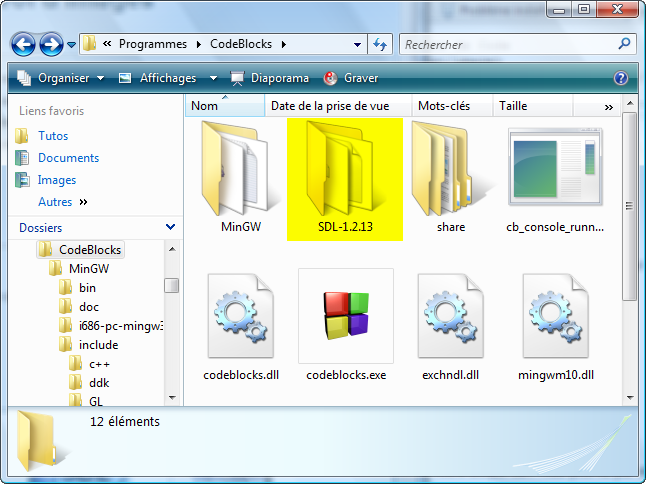
\includegraphics[width=0.8\textwidth]{Chapter_III-1_SDL-folder}
\end{figure}


بالنسبة لي فإن المسار هو التالي :

\InlineCode{C:\textbackslash Program Files (x86)\textbackslash CodeBlocks\textbackslash SDL-1.2.13}

احفظ المسار الذي به البرنامج، ستحتاج إليه عندما تريد تعديل إعدادات 
\textenglish{Code::Blocks}
لاحقا.

و الآن، علينا بالقيام بخطوة بسيطة، لتسهيل الأمور علينا، توجّه إلى المسار
\InlineCode{include/SDL}
(في حالتي، هو متواجد بـ\InlineCode{C:\textbackslash Program Files (x86)\textbackslash CodeBlocks\textbackslash SDL-1.2.13\textbackslash include\textbackslash SDL})،
قم بنسخ الملفات الرأسية
\InlineCode{.h}
 في المجلّد الأب، (أي في :\\ 
\InlineCode{C:\textbackslash Program Files (x86)\textbackslash CodeBlocks\textbackslash SDL-1.2.13\textbackslash include}).

\begin{figure}[H]
	\centering
	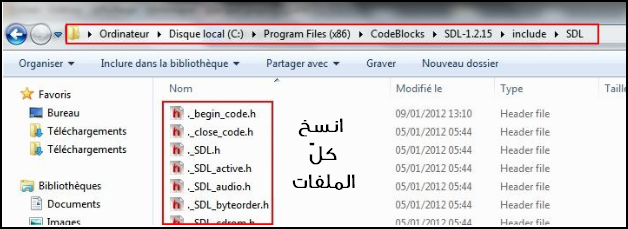
\includegraphics[width=0.8\textwidth]{Chapter_III-1_SDL-h-copy}
\end{figure}
\begin{figure}[H]
	\centering
	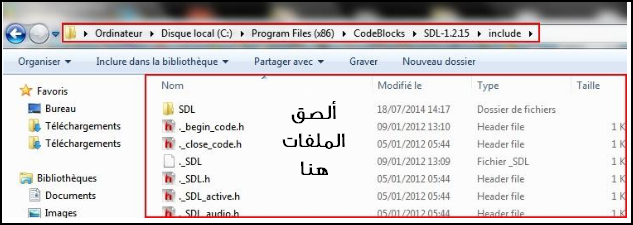
\includegraphics[width=0.8\textwidth]{Chapter_III-1_SDL-h-past}
\end{figure}

ها قد تم تسطيب المكتبة، فلنقم الآن بتعديل إعدادات
\textenglish{Code::Blocks}.

\subsubsection{إنشاء مشروع \textenglish{SDL}}

افتح
\textenglish{Code::Blocks}
و قم بإنشاء مشروع جديد.

\begin{figure}[H]
	\centering
	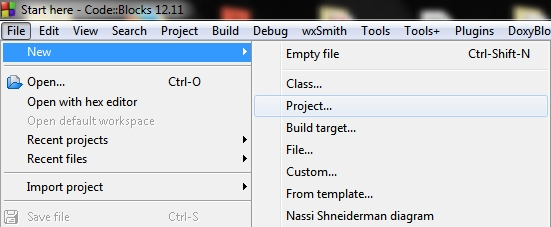
\includegraphics[width=0.7\textwidth]{Chapter_III-1_CodeBlocks-New-Project}
\end{figure}


عوض أن تقوم باختيار 
\textenglish{Console Application}
كما جرت العادة، اختر 
\textenglish{SDL project}.

\begin{figure}[H]
	\centering
	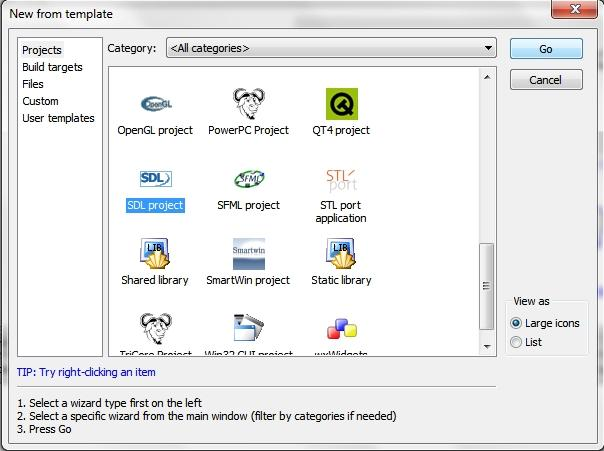
\includegraphics[width=0.8\textwidth]{Chapter_III-1_SDL-Project}
\end{figure}

النافذة الأولى لا جدوى منها، قم بتجاوزها بالضغط على "التالي"
(\textenglish{Next}).

\begin{figure}[H]
	\centering
	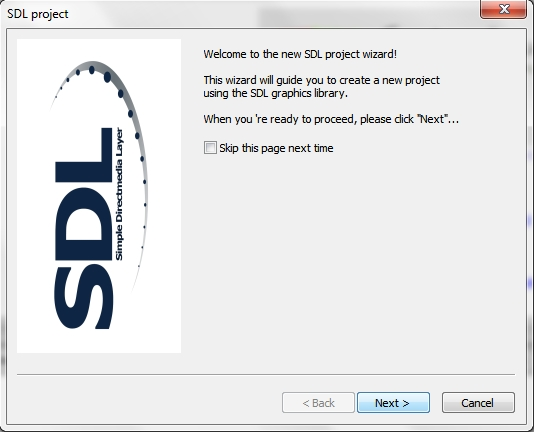
\includegraphics[width=0.8\textwidth]{Chapter_III-1_SDL-Project-Welcome}
\end{figure}

سيُطلب منك أن تقوم بإدخال اسم المشروع، قم بذلك كالعادة :

\begin{figure}[H]
	\centering
	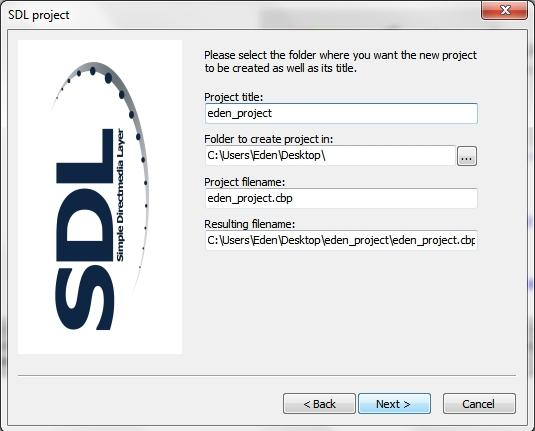
\includegraphics[width=0.8\textwidth]{Chapter_III-1_SDL-Project-path}
\end{figure}

الآن يجب اختيار المسار الذي ثبتنا فيه المكتبة :

\begin{figure}[H]
	\centering
	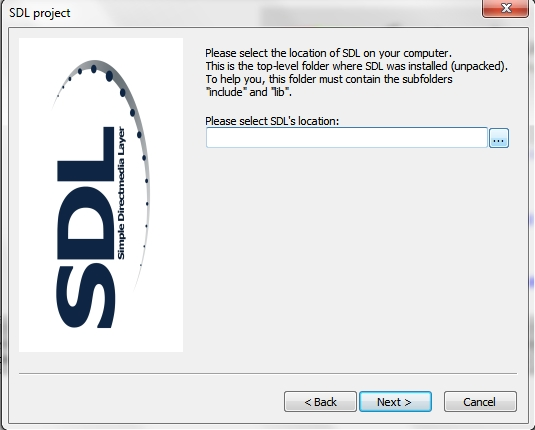
\includegraphics[width=0.8\textwidth]{Chapter_III-1_SDL-path}
\end{figure}

اضغط على الزر الذي يأخذ شكل مربّع به ثلاث نقاط، ستظهر لك النافذة التالية :

\begin{figure}[H]
	\centering
	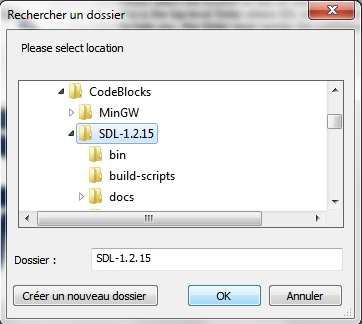
\includegraphics[width=0.5\textwidth]{Chapter_III-1_SDL-path-select}
\end{figure}

قم باختيار المسار (بالنسبة لي هو
\InlineCode{C:\textbackslash Program Files (x86)\textbackslash CodeBlocks\textbackslash SDL-1.2.13}).

قد تظهر لك في مكان النافذة السابقة هذه النافذة :

\begin{figure}[H]
	\centering
	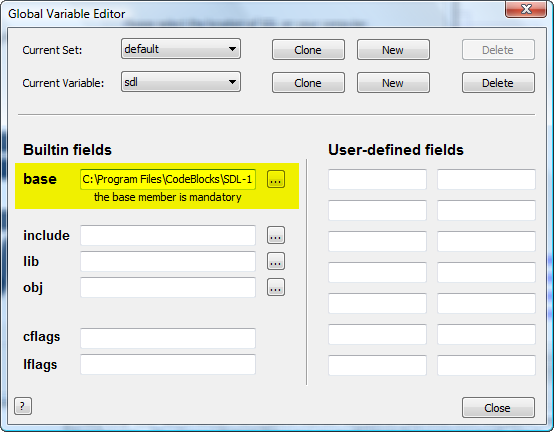
\includegraphics[width=0.75\textwidth]{Chapter_III-1_SDL-path-select-2}
\end{figure}

املأ الحقل
\textenglish{base}
بنفس الطريقة السابقة، ثمّ اضغط على زر الخروج، و ستلاحظ أن المسار قد تم تسجيله كالتالي :

\begin{figure}[H]
	\centering
	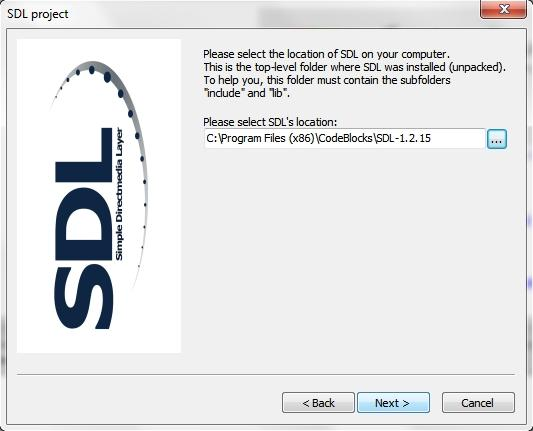
\includegraphics[width=0.8\textwidth]{Chapter_III-1_SDL-path-filled}
\end{figure}

اضغط على
\textenglish{Next}،
 ستظهر لك نافذة اختيار المترجم، قم باختيار الأوضاع
\textenglish{Realease}
أو
\textenglish{Debug}
(هذا لا يهم).

أخيرا اضغط على "إنهاء"
(\textenglish{Finish}).
 سيتم إنشاء المشروع التجريبي :
 
 \begin{figure}[H]
 	\centering
 	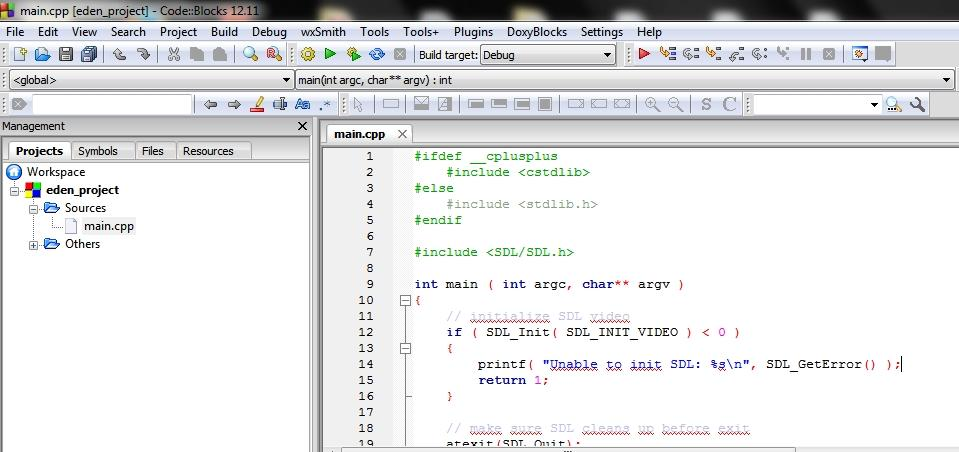
\includegraphics[width=\textwidth]{Chapter_III-1_SDL-test-project}
 \end{figure}


يحتوي المشروع على ملفين 
\InlineCode{main.cpp}
و ملف
\InlineCode{.bmp}
قبل أن تحاول القيام بالترجمة. يجب القيام بخطوة أخيرة (عليك القيام بها دائما)، و هي نسخ الملف 
\InlineCode{SDL.dll}
من ملفات المكتبة (الّذي يفترض أن يكون في المسار 
\InlineCode{C:\textbackslash Program Files (x86)\textbackslash CodeBlocks\textbackslash SDL-1.2.13\textbackslash bin\textbackslash SDL.dll})
و ضعه في المجلّد الخاص بالمشروع.

 \begin{figure}[H]
	\centering
	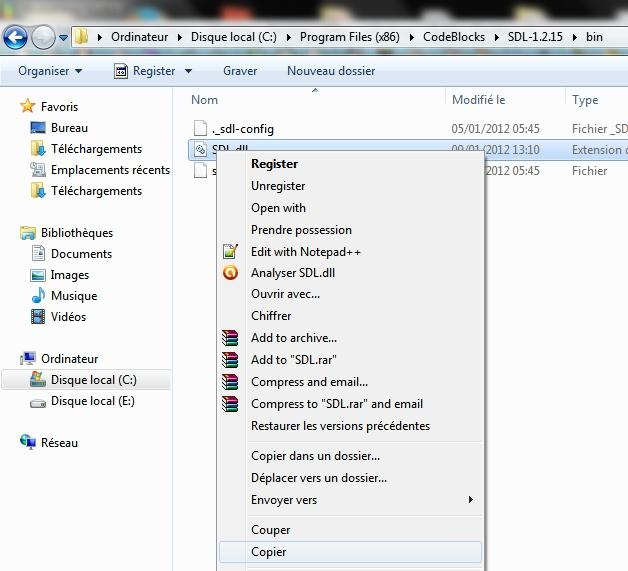
\includegraphics[width=0.8\textwidth]{Chapter_III-1_SDL-DLL-copy}
\end{figure}
 \begin{figure}[H]
	\centering
	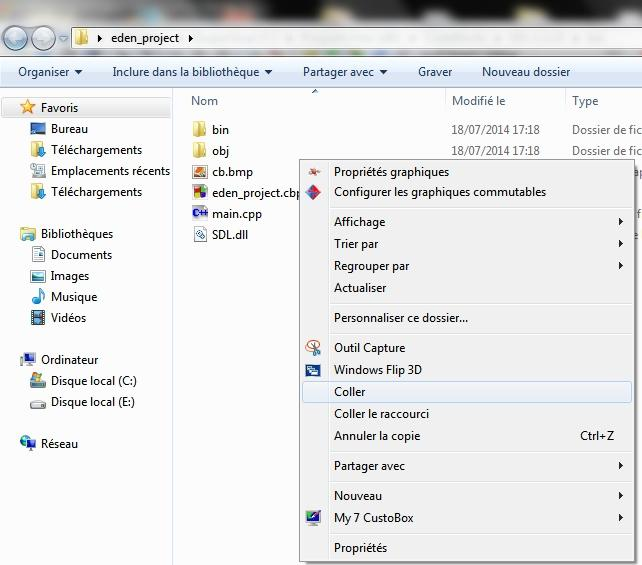
\includegraphics[width=0.8\textwidth]{Chapter_III-1_SDL-DLL-past}
\end{figure}

أخرج من 
\textenglish{Code::Blocks}
و أعد الدخول إليه، ثم قم بترجمة البرنامج المُقترح مسبقاً. يفترض أن تظهر النافذة التالية :

 \begin{figure}[H]
	\centering
	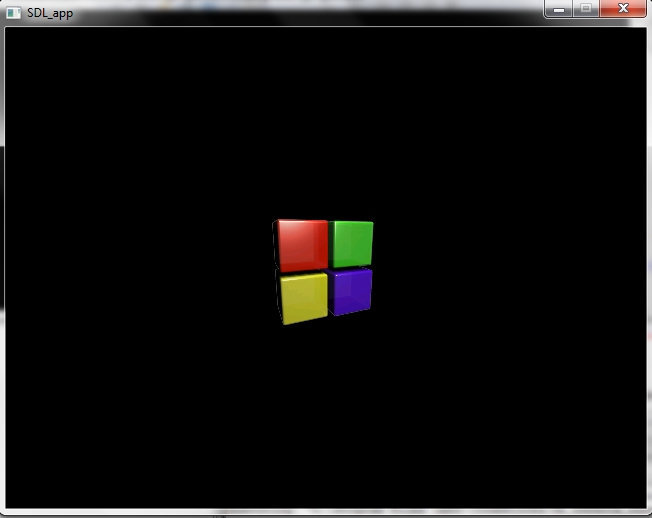
\includegraphics[width=0.8\textwidth]{Chapter_III-1_SDL-test-window}
\end{figure}


إذا ظهرت لك النافذة السابقة، فهنيئا لك، المكتبة مثبتة بشكل جيد !

\begin{information}
إن ظهرت لك الرسالة 
"\textenglish{The application can't start because the file SDL.dll is missing}"
أي أنه لا يمكن تشغيل البرنامج، لأن ملف 
\InlineCode{SDL.dll}
غير موجود، فهذا يعني أنك لم تقم بنسخ الملف الأخير في ملفات المشروع كما طلبت منك !\\
و كما قلت، إن كنت تريد تسليم المشروع إلى أصدقائك، عليك بارفاق الملف التنفيذي 
\InlineCode{.exe}
بالملف 
\InlineCode{SDL.dll}،
بينما أنت لست بحاجة إلى إعطائهم الملفات 
\InlineCode{.h}
و
\InlineCode{.a}
الّتي لا تهم أحدا سواك.
\end{information}

\begin{tcolorbox}[breakable,title=ملاحظات مترجمة الكتاب,colback=orange!20,colframe=orange!70,fontupper=\footnotesize,coltitle=white,fonttitle=\large]
كلّ الشرح الموجود في هذا الجزء يعطي الطريقة الّتي استخدمتها مترجمة الكتاب لتشغيل البرنامج في حالة ما لم تعمل الطريقة السابقة (الأصليّة). هذا يعني أنّ هذه الفقرات التالية ليست موجودة في الكتاب الفرنسي الأصلي، و إنّما هي مساهمة شخصيّة من المترجمة.
\tcblower

إن لم يشتغل البرنامج و لازال المترجم يشير دائما إلى عدم وجود الملف 
\InlineCode{SDL.dll}،
فجرب نسخ هذا الأخير و لصقه في المجلدين 
\textenglish{Debug}
و 
\textenglish{Release}
من مجلّد المشروع، أي في نفس المكان الذي يتواجد به الملف التنفيذي.

أريد أن أنوّهك بأن المشروع الذي تم انشاؤه هو خاص باللغة 
\textenglish{C++}
(لأنها اللغة التي يتم اختيارها تلقائيا من بيئة التطوير، كون أن هذه الأخيرة تم تطويرها للعمل بلغة الـ\textenglish{C++})،
سنقوم إذا بتحويل هذا المشروع من
\textenglish{C++}
إلى 
\textenglish{C}
ببساطة.\\
توجّه إلى ملفات المشروع، ستجد الملف
\InlineCode{main.cpp}
قم بتغيير اسمه إلى
\InlineCode{main.c}.

 \begin{figure}[H]
	\centering
	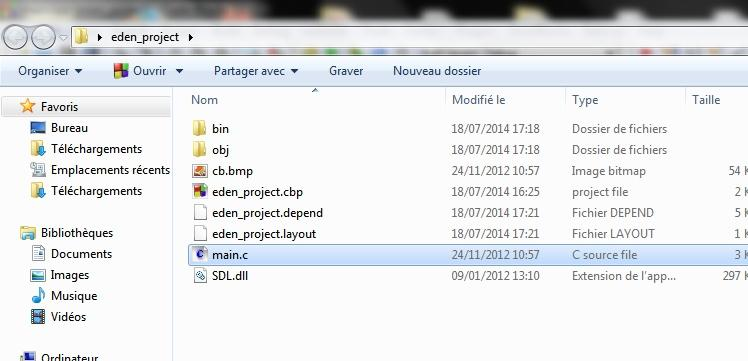
\includegraphics[width=\textwidth]{Chapter_III-1_SDL-rename}
\end{figure}

أدخل الآن إلى
\textenglish{Code::Blocks}،
ستظهر لك على الأرجح النافذة التالية :

 \begin{figure}[H]
	\centering
	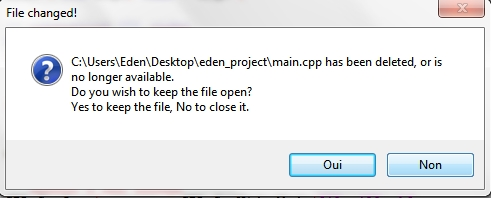
\includegraphics[width=0.7\textwidth]{Chapter_III-1_SDL-keep-open}
\end{figure}


اضغط على الزر "لا"
(\textenglish{No}).

توجه إلى القائمة اليسارية، و قم بالنقر باليمين على الملف
\InlineCode{main.cpp}
و اختر حذفه من المشروع :

\begin{figure}[H]
	\centering
	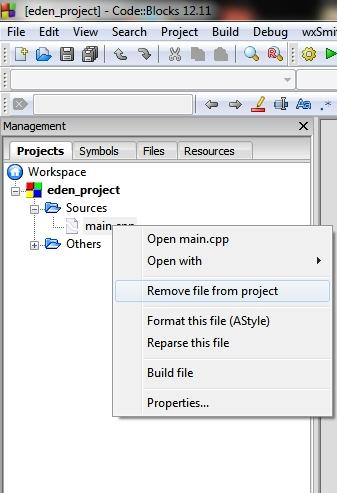
\includegraphics[width=0.4\textwidth]{Chapter_III-1_SDL-remove-cpp}
\end{figure}

اضغط على اسم المشروع، و اطلب إضافة ملف جديد :

\begin{figure}[H]
	\centering
	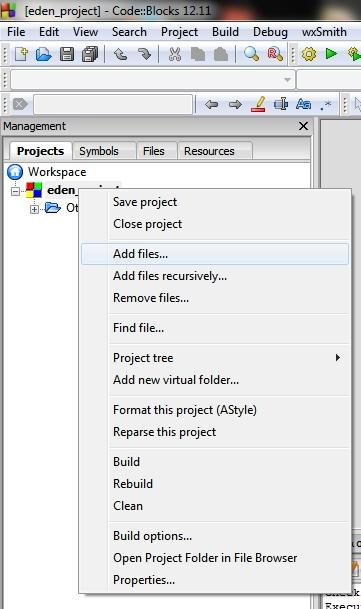
\includegraphics[width=0.4\textwidth]{Chapter_III-1_SDL-add}
\end{figure}

اختر الملف
\InlineCode{main.c}
من ملفات المشروع :

\begin{figure}[H]
	\centering
	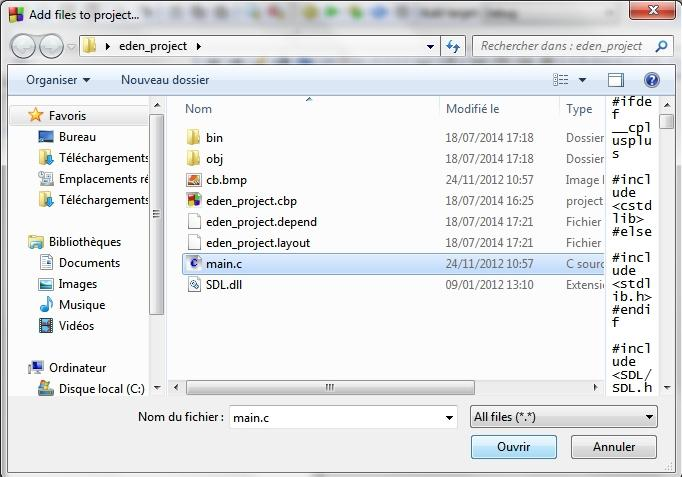
\includegraphics[width=0.8\textwidth]{Chapter_III-1_SDL-mainc}
\end{figure}

ستظهر لك نافذة أخرى، قم باختيار
\textenglish{Next}،
ثم انقر على "موافق"
(\textenglish{OK}).

\begin{figure}[H]
	\centering
	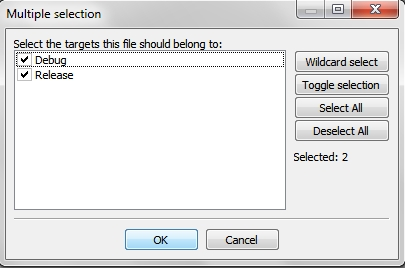
\includegraphics[width=0.6\textwidth]{Chapter_III-1_SDL-selection}
\end{figure}

أنقر باليمين مجددا على الملف 
\InlineCode{main.c}
و اختر "خصائص" 
(\textenglish{Properties}) :

\begin{figure}[H]
	\centering
	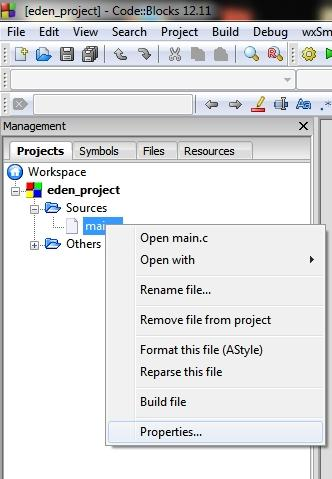
\includegraphics[width=0.5\textwidth]{Chapter_III-1_SDL-file-properties}
\end{figure}

توجه إلى القائمة
\textenglish{Advanced}،
ستجد
\textenglish{Compiler variable}،
غيّرها من
\textenglish{CPP}
إلى
\textenglish{CC}
كالتالي :

\begin{figure}[H]
	\centering
	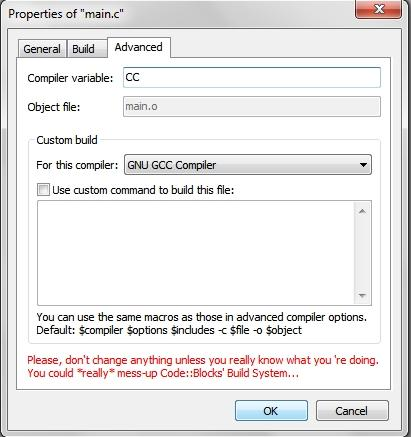
\includegraphics[width=0.7\textwidth]{Chapter_III-1_SDL-file-properties-advanced}
\end{figure}

اضغط بعد ذلك على
\textenglish{OK}
هذا ما سيبدو عليه المشروع الجديد :

\begin{figure}[H]
	\centering
	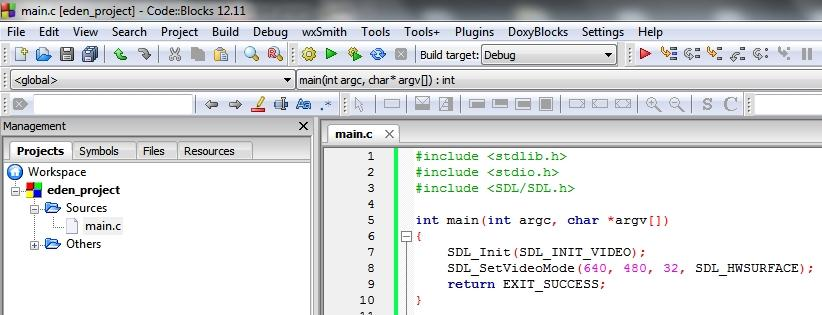
\includegraphics[width=\textwidth]{Chapter_III-1_SDL-new-file}
\end{figure}

ضع الشفرة التالية بدل الشفرة السابقة :

\begin{Csource}
#include <stdlib.h> 
#include <stdio.h> 
#include <SDL/SDL.h>
int main(int argc, char *argv[]) 
{ 
	SDL_Init(SDL_INIT_VIDEO); 
	SDL_SetVideoMode(640, 480, 32, SDL_HWSURFACE); 
	return EXIT_SUCCESS; 
}
\end{Csource}

و أخيراً، من القائمة العلوية، اختر هدف البناء 
\InlineCode{Release}.

\begin{figure}[H]
	\centering
	
\includegraphics[width=0.4\textwidth]{Chapter_III-1_SDL-build-target}
\end{figure}


يمكنك ترجمة البرنامج، ستظهر لك نافذة و تختفي فجأة، لا تقلق، سنعالج ذلك لاحقاً، أنا أهنّئك، كل شيء يعمل بشكل جيد جدا.

\end{tcolorbox}

يمكنك مسح الملف 
\InlineCode{.bmp}
لأننا لسنا بحاجة إليه. بالنسبة للملف 
\InlineCode{main.c}، 
يمكنك الآن استبدال محتواه بالشفرة التالية :

\begin{Csource}
#include <stdlib.h>
#include <stdio.h>
#include <SDL/SDL.h>
int main(int argc, char *argv[])
{
	return 0;
}
\end{Csource}
إنها شفرة مبدئية، تشبه الشفرات التي تعوّدنا عليها (تضمين
\InlineCode{stdlib.h}
و
\InlineCode{stdio.h}
ثم 
\InlineCode{main}).
الشيء الوحيد الذي تغيّر هو تضمين الملف
\InlineCode{SDL.h}.
إنّه ملف رأسيّ يستكلف نفسه بتضمين كل الملفات الرأسية الخاصة بالمكتبة 
\textenglish{SDL}.

\subsection{إنشاء مشروع \textenglish{SDL} في \textenglish{Visual C++}}

\subsubsection{استخراج ملفات الـ\textenglish{SDL}}

من الموقع الرسمي، قم بتنزيل آخر نسخة من المكتبة من قسم
"\textenglish{Development Libraries}"
و اختر نسخة
\textenglish{Visual C++ 2005 Service Pack 1}.

افتح الملف
\InlineCode{.zip}.\\
إنه يحتوي  على التوثيق (في المجلد
\InlineCode{docs})،
 الملفات
\InlineCode{.h}
(في المجلد
\InlineCode{include})، 
و الملفات
\InlineCode{.lib}
(في المجّلد
\InlineCode{lib})
المكافئة للملفات
\InlineCode{.a}
بالنسبة لمترجم
\textenglish{Visual}.
ستجد أيضاً الملف 
\InlineCode{SDL.dll}
في المجلّد
\InlineCode{lib}.

\begin{itemize}
	\item انسخ الملف
	\InlineCode{SDL.dll}
	إلى مجلّد المشروع.
	\item انسخ الملفات
	\InlineCode{.lib}
	إلى المجلّد 
	\InlineCode{lib}
	الخاص بـ\textenglish{Visual C++}.
	بالنسبة لي، أنا أتكلم عن المجلّد
	
	\InlineCode{C:\textbackslash Program Files (x86)\textbackslash Microsoft Visual Studio 8\textbackslash VC\textbackslash lib}.
	
	\item انسخ الملفات
	\InlineCode{.h}
	إلى المجلّد
	\InlineCode{includes}
	الخاص بـ\textenglish{Visual C++}.
	أنشئ مجلّدا
	\InlineCode{SDL}
	في المجلد
	\InlineCode{includes}
	لجمع الملفات
	\InlineCode{.h}
	الخاصة بالـ\textenglish{SDL}
	فيه. بالنسبة لي، سأضع تلك الملفات في المجلد :
	
	\InlineCode{C:\textbackslash Program Files (x86)\textbackslash Microsoft Visual Studio 8\textbackslash VC\textbackslash include\textbackslash SDL}.

\end{itemize}

\subsubsection{إنشاء \textenglish{SDL} مشروع جديد}

في الـ\textenglish{Visual C++}
أنشئ مشروعاً من نوع 
\textenglish{Application console Win32}.
سمّه مثلاً
\InlineCode{testsdl}
ثم اضغط على "موافق".

ستفتح نافذة مساعدة. توجه إلى 
\textenglish{Application parameters}
و تأكد من أن الخانة
\InlineCode{Empty project}
مختارة.

\begin{figure}[H]
	\centering
	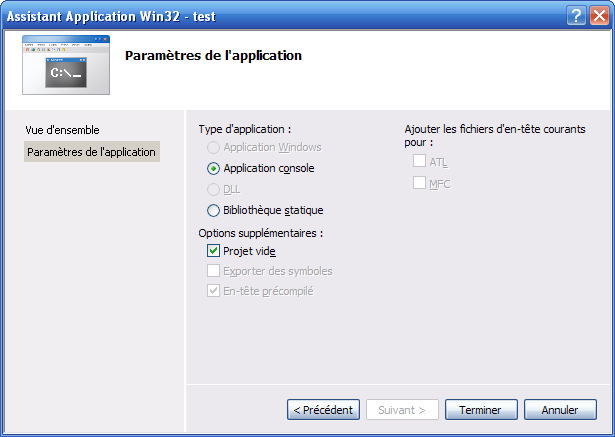
\includegraphics[width=0.8\textwidth]{Chapter_III-1_VisualCpp-Assistant}
\end{figure}

لقد تمّ إنشاء المشروع إذا. إنّه فارغ. أضف إليه ملفاً جديداً و ذلك بالنقر على
\InlineCode{Source files}
ثم
\InlineCode{Add}
ثم
\InlineCode{New element} :

\begin{figure}[H]
	\centering
	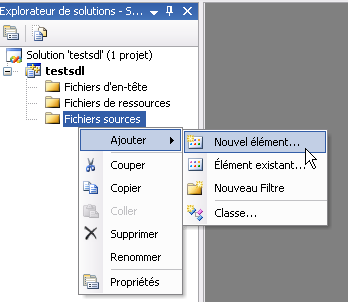
\includegraphics[width=0.5\textwidth]{Chapter_III-1_VisualCpp-Add}
\end{figure}

حينما تفتح نافذة جديدة، أطلب إنشاء ملف جديد من نوع
\InlineCode{C++ File (.cpp)}،
قم بتسميته
\InlineCode{main.c}.
بوضعك للامتداد
\InlineCode{.c}
فإن الـ\textenglish{Visual}
سيقوم بانشاء ملف
\textenglish{C}
و ليس
\textenglish{C++}.

أكتب (أو انسخ/ألصِق) الشفرة المبدئية الذي وضعتها أعلاه، في الملف الجديد الذي أنشأته.

\subsubsection{تخصيص مشروع \textenglish{SDL} في \textenglish{Visual C++}}

التعديل على المشروع أصعب قليلاً مما هو الحال مع الـ\textenglish{Code::Blocks}،
لكن بقليل من التركيز، ستتمكن من فعله. توجّه إلى خصائص المشروع من
\InlineCode{Project} / \InlineCode{testsdl properties}.

\begin{itemize}
	\item في القسم
	\InlineCode{C / C++} / \InlineCode{Code generation}
	عدّل قيمة الـ\InlineCode{Runtime Libraries}
	إلى\\
	\InlineCode{DLL multithread (/MD)}.
	\item في القسم 
	\InlineCode{C / C++} / \InlineCode{Advanced}
	اختر
	\InlineCode{Compilation as}
	و ضع القيمة\\
	\InlineCode{Compile as C code (/TC)}
	(و إلا فإن
	\textenglish{Visual}
	سيترجم البرنامج كأنه ملف
	\textenglish{C++}
	و ليس كملف
	\textenglish{C}).
	\item في القسم  
	\InlineCode{Link editor} / \InlineCode{Input}
	عدّل قيمة الـ\InlineCode{Additional dependencies}
	لكي تضيف
	\InlineCode{SDL.lib}
	و
	\InlineCode{SDLmain.lib}.
	\item في القسم
	\InlineCode{Link editor} / \InlineCode{System}
	عدّل قيمة الـ\InlineCode{Sub-System}
	إلى الـ\InlineCode{Windows}.
\end{itemize}

\begin{figure}[H]
	\centering
	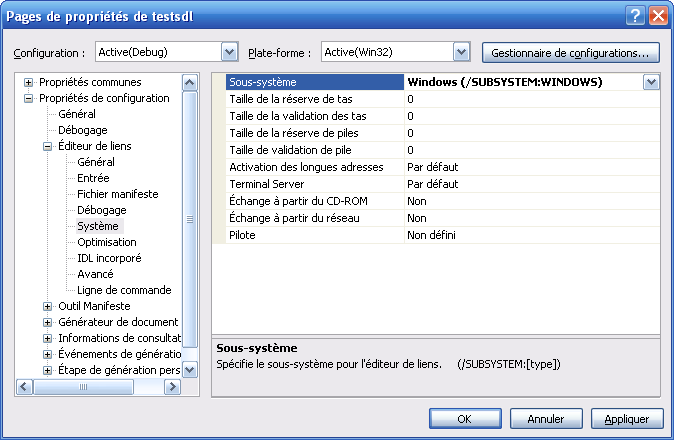
\includegraphics[width=0.8\textwidth]{Chapter_III-1_VisualCpp-project-properties}
\end{figure}


قم بالضغط على "موافق" لحفظ التغييرات.\\
يمكنك الآن الترجمة و ذلك بالذهاب إلى
\InlineCode{Generate}
ثم
\InlineCode{Generate solution}.

ستجد الملف التنفيذي الذي يتواجد بمجلد المشروع (أو بمجلد داخلي يسمى
\InlineCode{Debug})
و لا تنس أنه على الملف
\InlineCode{SDL.dll}
أن يتواجد في نفس المجلّد الذي يتواجد به الملف التنفيذي. أنقر مرّتين على
\InlineCode{.exe}،
 إذا سار كلّ شيء على ما يرام، فلن يحصل أيّ شيء، و إلّا فسيحدث خطأ إذا لم يكن الملف
\InlineCode{SDL.dll}
في نفس المجلّد.

\section{إنشاء مشروع \textenglish{SDL} : \textenglish{Mac OS} (\textenglish{Xcode})}

فلتقم بتنزيل النسخة 1.2 من الـ\textenglish{SDL}،
و ذلك من خلال الجزء
"\textenglish{Download}"
أسفل يسار الموقع، كالتالي :

\begin{figure}[H]
	\centering
	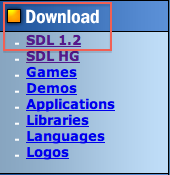
\includegraphics[width=0.25\textwidth]{Chapter_III-1_SDL-Mac-Download}
\end{figure}

في أسفل الصفحة ستجد قسماً يدعى 
"\textenglish{Runtime Libraries}".
نزّل الملف الذي يتناسب مع هندسة معالج جهازك
(\textenglish{Intel} أو \textenglish{PowerPC})،
 هذا ما ستوضحه الصورة الموالية. إن كنت تريد معرفة هندسة المعالج، يمكنك الذهاب إلى القائمة 
"\textenglish{Apple}"
في أعلى اليسار، و النقر على 
"\textenglish{About this Mac}".
في السطر 
"\textenglish{Processor}"
ستجد إما
\textenglish{Intel} أو \textenglish{PowerPC}.

\begin{figure}[H]
	\centering
	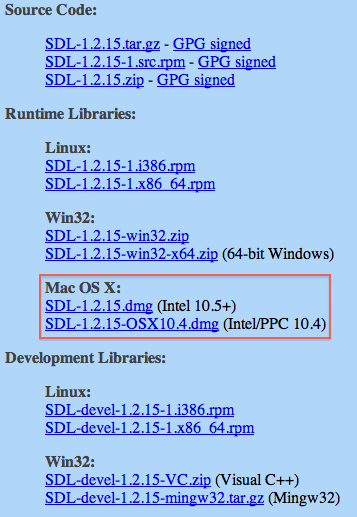
\includegraphics[width=0.5\textwidth]{Chapter_III-1_SDL-Mac-Download-version}
\end{figure}

حينما يتم تنزيل الملف، انقر عليه مرتين، يفترض أن يفتح لوحده. ستجد بهذا المجلّد مجلّدا
\InlineCode{SDL.framework}
قم بنسخه و لصقه في المجلد 
\InlineCode{/Library/Frameworks}.

إنتهى، المكتبة مسطّبة الآن !\\
ستجد مجلّدا آخر اسمه 
\InlineCode{devel-lite}
أتركه مفتوحا، سنعود إليه لاحقاً.

الآن قم بانشاء مشروع جديد
"\textenglish{Cocoa Application}"،
اضغط على
"\textenglish{Next}".
في 
\InlineCode{Product Name}
قم بتسمية المشروع (كـ"\textenglish{SDL}"
مثلاً). و في 
\InlineCode{Company Identifier}،
ضع ما تريد (كاسم مستعار لك مثلا). أترك الباقي كما هو ثم اضغط على 
"\textenglish{Next}".
اختر أين تريد وضع المشروع. سيتم إنشاء مجلّد بطريقة تلقائية و ليس عليك إنشاء واحد بنفسك ووضع ملفات المشروع بداخله.

ما إن يتم إنشاء المشروع، قم بالتخلص من الملفات التي لا تحتاجها :
\InlineCode{AppDelegate.h}، \InlineCode{AppDelegate.m}، \InlineCode{MainMenu.xib}، \InlineCode{InfoPlist.strings}، \InlineCode{main.m} و \InlineCode{Credits.rtf} :

\begin{figure}[H]
	\centering
	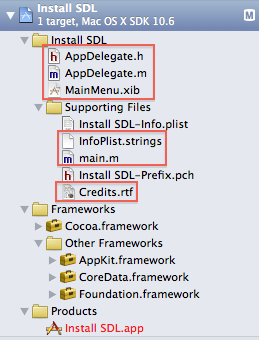
\includegraphics[width=0.5\textwidth]{Chapter_III-1_SDL-project-unused-files}
\end{figure}

اختر المشروع من التفرع الشجري اليساري (القسم
\InlineCode{Install SDL}
من الصورة الموالية) في الشجرة الثانية اختر اسم مشروعك من قسم 
\InlineCode{PROJECT}
و ليس من
\InlineCode{TARGETS} :

\begin{figure}[H]
	\centering
	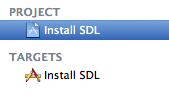
\includegraphics[width=0.3\textwidth]{Chapter_III-1_Xcode-SDL-project}
\end{figure}

يمكنك أيضاً تغيير الـ\textenglish{localisation}
من 
\InlineCode{English}
إلى 
\InlineCode{French}.
اختر 
\InlineCode{English}،
أنقر على
\InlineCode{-}
للمسح و على 
\InlineCode{+}
لإضافة 
\InlineCode{French}،
هذا يعود إليك و لست مضطراً للقيام بذلك.

سنقوم الآن بتخصيص المشروع على نظام
\textenglish{32 bits}
( لأن المكتبة لا تشتغل على أنظمة
\textenglish{64 bits})،
و سنقوم بإضافة المسارات من أجل الـ\textenglish{frameworks}،
و للملفات الرأسية أيضاً. اضغط على
\InlineCode{Build Settings}
ثم 
\InlineCode{All}
ثم في 
\InlineCode{Architectures}
انقر على
\InlineCode{64-bit Intel}
 و اختر
\InlineCode{32-bit Intel} :

\begin{figure}[H]
	\centering
	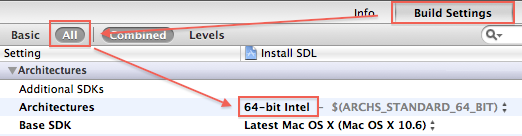
\includegraphics[width=0.8\textwidth]{Chapter_III-1_Xcode-SDL-build-setting}
\end{figure}


ما إن تفعل ذلك، اختر
\InlineCode{LLVM GCC 4.2}
من السطر
\InlineCode{Compiler for C/C++/Objective-C}.

\begin{figure}[H]
	\centering
	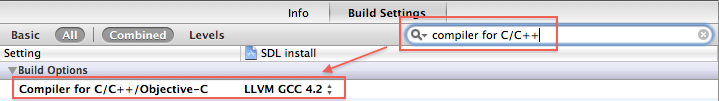
\includegraphics[width=0.8\textwidth]{Chapter_III-1_Xcode-gcc}
\end{figure}

اذهب إلى منطقة البحث في أعلى اليمين، و اكتب
"\textenglish{search paths}"،
يجدر بك أن تجد سطرين مهمّين بالنسبة لنا و هما
\InlineCode{Header search paths}
و 
\InlineCode{Framework search paths}.
انقر مرتين على الجهة اليمنى للسطر 
\InlineCode{Framework search paths}
أنقر على علامة
\InlineCode{+}
 و أضف المسار
\InlineCode{/Library/Frameworks}.
بالنسبة للسطر 
\InlineCode{Header Search paths}
أضف المسار\\
\InlineCode{/Library/Frameworks/SDL.framework/Headers}.

\begin{figure}[H]
	\centering
	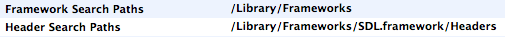
\includegraphics[width=0.8\textwidth]{Chapter_III-1_Xcode-SDL-framework}
\end{figure}

اختر الآن "هدفك"، و هذه المرة من قسم 
\InlineCode{TARGETS} :

\begin{figure}[H]
	\centering
	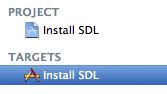
\includegraphics[width=0.3\textwidth]{Chapter_III-1_Xcode-SDL-target}
\end{figure}

توجه إلى 
\InlineCode{Summary}،
في المنطقة
\InlineCode{Application Category}
يمكنك وضع ما تشاء، لن يغير هذا شيئا كبيراً، لأنه ينفع من أجل الـ\textenglish{AppStore}
فقط. عدّل السطر 
\InlineCode{Main Interface}
و ضع 
"\textenglish{SDLMain}".
بالنسبة للـ\InlineCode{App Icon}
فاسمه يدل عليه، فهو يسمح لك بتحديد أيقونة لبرنامجك. يكفي سحب ثم تحرير الصورة المُراد استعمالها كأيقونة. بالنسبة للمنطقة 
\InlineCode{Linked Frameworks and Libraries}
سنقوم بإضافة الـ\textenglish{framework}
الخاص بنا
\InlineCode{SDL.framework}،
أنقر على
\InlineCode{+}
في منطقة البحث ، أكتب 
"\textenglish{SDL}"،
حين تجده في القائمة، أنقر على 
\InlineCode{Add}،
إن لم تجده فهذا يعني أنك لم تقم بوضعه في المجلّد المناسب 
(\InlineCode{/Library/Frameworks}).

\begin{information}
الأيقونات في
\textenglish{Mac OS}
هي بصيغة
\InlineCode{.icns}.
إن استعملت صيغة أخرى فستلاحظ أن الأيقونة لا تظهر. إن أردت تحويل صيغة صورة عادية إلى أيقونة استعمل برنامج 
\textbf{\textenglish{Icon Composer}}.
المتواجد في المجلد
\InlineCode{/Developer/Applications/Utilities}،
يكفي أن تسحب الأيقونة إلى المربع المخصص لها ثم تحفظها.
\end{information}

في المنطقة 
\InlineCode{Info}
يمكننا أن نشير إلى العديد من المعلومات في البرنامج، يمكنك الإطلاع عليها أكثر من خلال قراءة الملفات التوثيقية الخاصة بـ\textenglish{Apple}.
الشيء الوحيد الذي يمكنك التعديل عليه هو 
\InlineCode{Localization}
من 
\InlineCode{en}
إلى 
\InlineCode{fr}،
كما يمكنك تعديل الـ\InlineCode{Copyright}
و وضع ما تريد.

توجّه الآن إلى 
\InlineCode{Build Phases}
و انقر على 
\InlineCode{Add Build Phase} / \InlineCode{Copy Files}
في أسفل يمين النافذة، اضغط على 
\InlineCode{Copy Files}
و غيّره إلى 
\InlineCode{Copy frameworks into app}.
في 
\InlineCode{Destination}
اختر
\InlineCode{Frameworks}
لتضيف الخاصة بك، قم بسحبها من التفرع الشجري اليساري و افلاتها في المنطقة
\InlineCode{Build phase}،
كما يظهر بالصورة  :

\begin{figure}[H]
	\centering
	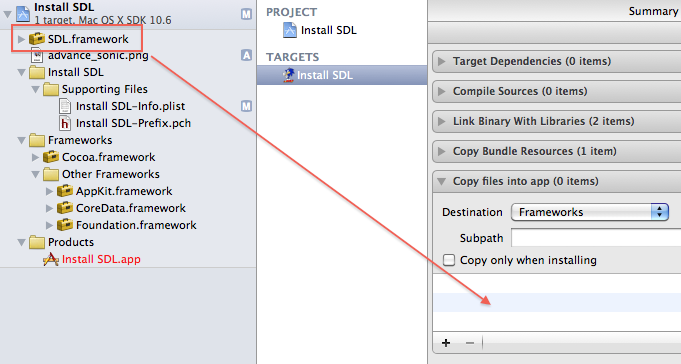
\includegraphics[width=\textwidth]{Chapter_III-1_Xcode-drop-framework}
\end{figure}

أنصحك بترتيب كل الـ\textenglish{frameworks}
الخاص بك في مجلد 
\InlineCode{Framework}
و هذا لكي يسهل عليك إيجادها.\\
و أيضاً بالنسبة للشفرات المصدرية، أنصحك بترتيبها في مجلدات ليسهل الوصول إليها. لإنشاء مجلد انقر باليمين على الشجرة اليسارية و اختر
\InlineCode{New Group}
ثم اسحب الملفات إلى داخلها.

سنقوم الآن بإضافة الملفات
\InlineCode{SDLMain.h}
و 
\InlineCode{SDLMain.m}،
توجه إلى المجلد 
\InlineCode{devel-lite}
المفتوح مسبقا و قم بإضافة الملفين إلى المشروع. إذا ظهرت لك نافذة تحديد خصائص النسخ، قم باختيار\\
\InlineCode{Copy items into destination group's folder (if needed)}.

آخر شيء : أنشئ ملفا
\InlineCode{main.c}.
توجه إلى القائمة 
\InlineCode{File} / \InlineCode{New} / \InlineCode{New File}
ثم إلى 
\InlineCode{C and C++}، 
اختر
\InlineCode{C File}
ثم
"\textenglish{Next}".
قم بتسمية الملف و هاقد أكملت.

\section{إنشاء مشروع \textenglish{SDL} :  \textenglish{GNU/Linux}}

لمن يستعملون بيئة تطويرية من أجل الترجمة، فعليهم بتغيير خواص المشروع (فالعملية مشابهة لما كنت قد شرحت). بالنسبة لمن يستعمل
\textenglish{Code::Blocks}،
فالطريقة هي نفسها التي شرحتها سابقاً.

\begin{question}
 ماذا عن الذين يقومون بترجمة الشفرات يدويا ؟
\end{question}

قد يوجد بين القراء من اعتاد على ترجمة الشفرات يدويا بالاستعانة بـ\textenglish{Makefile}
(ملف يساعد على عملية الترجمة).\\
إذا كانت هذه حالتك، فأدعوك لتحميل
\textenglish{Makefile}
الّذي يُمكن أن يُستخدم لترجمة مشاريع الـ\textenglish{SDL}.

\url{http://www.siteduzero.com/uploads/fr/ftp/mateo21/makefile_sdl}

الشيء الوحيد المختلف، هو إضافة المكتبة
\textenglish{SDL}
إلى محرّر الروابط
(\InlineCode{LDFLAGS}).
يجدر بك أن تكون قد نزّلت المكتبة و ثبّتها في مجلّد ملفات المترجم، بنفس طريقة
\textenglish{Windows}
(المجلدان
\InlineCode{include/SDL}
و 
\InlineCode{lib}).

بعد ذلك يجب عليك أن تكتب الأوامر التالية في الكونسول :

\begin{Console}
make      	# To compile the project
make clean	# To delete compilation files (useless .o files)
make mrproper	# To delete all files except source ones
\end{Console}

\section*{ملخّص}

\begin{itemize}
	\item الـ\textenglish{SDL}
	مكتبة منخفضة المستوى، تسمح بإنشاء نوافذ و التعامل مع الرسوميات
	\textenglish{2D}.
	\item المكتبة ليست مسطّبة تلقائيا في الحاسوب، يجب عليك أن تنزّلها بنفسك و تقوم بتخصيص البيئة التطويرية لتعمل معها.
	\item المكتبة حرة و مجّانية، مما يسمح باستعمالها السريع و الدائم.
	\item توجد آلاف المكتبات الأخرى، و كثير منها ذو جودة عالية جداً. و قد تم اختيار المكتبة 
	\textenglish{SDL}
	لبقيّة هذا الكتاب لأجل سهولتها. لمن يريد بناء واجهات رسومية بنوافذ، أزرار و قوائم، فأنا أنصحه بالمكتبة 
	\textenglish{GTK+}
	مثلا.
\end{itemize}
